\subsection{Our proposed pointing strategies}
\label{sec:proposed_pointings}
Given the constraints outlined in Sec.~\ref{sec:constraints_on_pointings} and the additional (non-physical) constraint of a single year's observing time, we select the following options for further study:

\begin{figure*}[ht]
	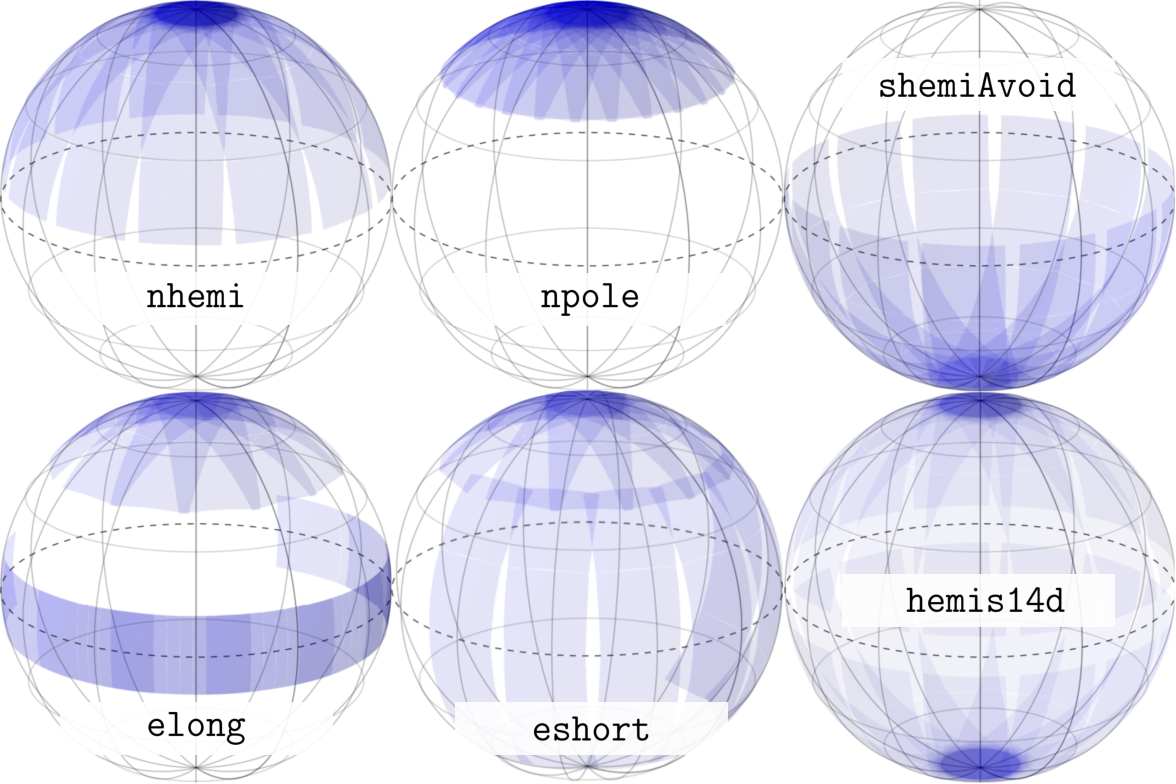
\includegraphics{figures/proposed_pointings_texttt.pdf}
	\caption{Proposed pointing strategies for a \tess extended mission, visualized in ecliptic coordinates. \nhemi, \npole, \shemiAvoid, \elong, \eshort, and \hemis. Note for \elong\ and \eshort\ that Earth and moon crossings likely make an entire year looking at the ecliptic impractical (see Fig.~\protect\ref{fig:earth_moon_elong}).}
	\label{fig:proposed_pointings}
\end{figure*}

\begin{description}
	\item[Option 1.] Focus on the North Ecliptic Pole (hereafter, \npole). Note that the geometry of \tesss lens hood still suppresses incoming sunlight in this scenario. 
	\textit{Justification:} maximizes average observing baseline per star; longest period coverage.
	\item[Option 2.] Repeat observations of the northern hemisphere (\nhemi).
	\textit{Justification:} `two-survey' strategy used for primary mission -- long survey at the North Ecliptic Pole; also gets fresh ephemerides at low ecliptic latitudes. Can phase in longitude to cover `gaps' from primary.
	\item[Option 3.] Repeat year 1 in the southern hemisphere, but with all fields 6 degrees further north in ecliptic latitude (\shemiAvoid).
	\textit{Justification:} covers most of sky missed in primary survey, freshens ephemerides \& avoids Earth-Moon crossings that would happen with this same strategy inverted in the North.
	\item[Option 4.] 7 sectors (14 orbits) with \tesss long axis along the ecliptic, 6 sectors focused at the North Ecliptic Pole (\elong).
	\textit{Justification:} covers sky missed in primary survey with $\sim3$ orbits of observing time per star on the ecliptic, opportunity of K2 follow-up, can be extended for longer period coverage, avoids Earth-Moon crossings.
	\item[Option 5.] 7 sectors with \tesss short axis along the ecliptic, 6 sectors focused at the North Ecliptic Pole (\eshort). 
	\textit{Justification:} similar to \elong, with slightly better ability to follow-up on \tess objects of interest (TOIs).
	\item[Option 6.] Cover both northern and southern ecliptic hemispheres in a year, by switching between northern and southern hemisphere sectors every $\sim13.7\ \text{day}$ orbit (\hemis).
	\textit{Justification:} freshen ephemeris times for most TOIs, faster than any other scenario.
\end{description}

In selecting these options for further study, we omitted other possible scenarios that will remain of interest, for instance in a fourth year of observing. We comment on these options and justify their omission from detailed calculations below:

\begin{itemize}
	\item Focus on the South Ecliptic Pole: omitted for simplicity (complement of \npole).
	\item Repeat observations of the southern hemisphere: omitted for simplicity (complement of \nhemi).
	\item Repeat year 2 in the northern hemisphere, but 6 degrees further south in ecliptic latitude: omitted for simplicity (complement of \shemiAvoid), and also due to Earth/Moon crossings (see Sec.~\ref{sec:earth_moon_crossings}).
	\item 1 year with \tesss long axis along the ecliptic. Omitted due to Earth/Moon crossings, which prevent detailed photometry for $\sim\!6\ \text{months/year}$.
	We show the outage as a function of time in Fig.~\ref{fig:earth_moon_elong}.
	\item 1 year with \tesss short axis along the ecliptic. Omitted due to Earth/Moon crossings, which prevent detailed photometry for $\sim 6\ \text{months/year}$.
	\item Cover both northern and southern ecliptic poles over a year, by switching between hemispheres every spacecraft orbit. Omitted because an important justification for this scenario -- refined ephemeris times, described in Sec.~\ref{sec:ephemeris_timing_analytic} -- suffers compared to \hemis.
	\item Monthly-specific scenarios. For instance, in the \nhemi\ scenario, during a month when the Earth or Moon crosses through the field of a camera pointed close to the ecliptic, tilt all the cameras away from the ecliptic as in the \npole\ scenario. Omitted for simplicity.
\end{itemize}


All of these potential spacecraft pointings, both selected and omitted, meet the constraint of having \tesss cameras point anti-Sun throughout the year, while also allowing the solar panels to collect sunlight.